\documentclass[12pt]{article}
\usepackage{amsmath}
\usepackage{amsfonts}
\usepackage{amssymb}
\usepackage{xfrac}
\usepackage{graphicx}
\usepackage[margin=0.5in]{geometry}

\begin{document}
\Large{\textbf{{\centerline{Fluid Mechanics}}}}
\smallskip
\small{\em{Rutuj Shah} \hfill \em{August'14}}
\bigskip
\noindent\makebox[\linewidth]{\rule{\paperwidth}{0.4pt}} %line spanning the entire page
\normalsize{\textbf{Intro to fluids}}
\begin{itemize}
\item Knudsen Number: \quad $\lambda = \frac { { k }_{ B }T }{ \sqrt { 2 } \pi { d }^{ 2 }P } $ , ${ K }_{ n } = \frac { \lambda  }{ L } $ , ${ K }_{ n }\le 0.01$ for continuum
\item Rate of Shearing Strain: \quad $\dot { \gamma  } =\frac { d\beta  }{ dt } =\frac { du }{ dy } $
\item Shearing Stress: \quad $\tau =\mu \dot { \gamma  } $ \quad for Newtonian Fluids
\item Kinematic Viscosity: \quad $\nu =\frac { \mu  }{ \rho  } $
\item Reynold's Number: \quad$\frac { \rho VD }{ \mu  } $
\item Sutherland Equation (gases): \quad$\mu  = \frac { C{ T }^{ \sfrac { 3 }{ 2 }  } }{ T + S } $
\item Andrade Equation (liquids): \quad $\mu  = D{ e }^{ \frac { B }{ T }  }$
\item Bulk Modulus: \quad$\quad{ E }_{ v }=-\frac { dp }{ \sfrac { dV }{ V }  } =\frac { dp }{ \sfrac { d\rho  }{ \rho  }  } $\quad , Compressibility: \quad $\kappa =\frac { 1 }{ { E }_{ v } } $
\item For polytropic process $\frac { P }{ { \rho  }^{ x } } $ Bulk Modulus: ${ E }_{ v } = xP$
\item Speed of Sound: $c=\sqrt { \frac { dp }{ d\rho  }  } =\sqrt { \frac { { { E }_{ v } } }{ \rho  }  } =\sqrt { \gamma RT } $
\item Excess Pressure: \quad$p=\frac { 2T }{ R } $ \quad for Soap:\quad $p=\frac { 4T }{ R } $
\item Height in a capillary: \quad$h\quad =\frac { 2T\cos { \theta  }  }{ \gamma R } $ \quad($\gamma$ is specific wt.)\\

\end{itemize}
\normalsize{\textbf{Fluid statics}}
\begin{itemize}
\item For the wedge:\quad ${ P }_{ y }-{ P }_{ s }=\quad \rho \frac { \delta y }{ 2 } { a }_{ y }$, \quad ${ P }_{ z }-{ P }_{ s }=\quad \rho \frac { \delta z }{ 2 } { (a }_{ z }+g)$
\item Surface Force:\quad$\delta { F }_{ s }=\quad -\triangledown P(\delta x\delta y\delta z)$, \quad Body Force:\quad$\delta W=\quad -\gamma (\delta x\delta y\delta z)\hat { k } $
\item Using Newton's 2nd Law:\quad$-\triangledown P- \gamma \hat { k } = \rho \hat { a } $
\item Incompressible fluids:\quad${ P }_{ 2 }-{ P }_{ 1 }=\rho gh$,\quad For compressible fluids:\quad$\frac { dp }{ dz } = -\rho g = -\frac { pg }{ RT } $
\item Troposphere:\quad$T={ T }_{ a }-\beta z$
\item Resultant force ~ Centroid\quad$\int { ydA=\quad { y }_{ c }A } $,\quad Centre of pressure\quad${ y }_{ R }=\quad \frac { \int { { y }^{ 2 }dA }  }{ { y }_{ c }A } $
\item Centre of pressures:\quad${ y }_{ R }=\quad \frac { { I }_{ xc } }{ { y }_{ c }A } +{ y }_{ c }$,\quad${ x }_{ R }=\quad \frac { { I }_{ xyc } }{ { y }_{ c }A } +{ x }_{ c }$
\item Metacentric height:\quad$GM=\frac { { I }_{ 0 } }{ { V }_{ submerged } } -CG$
\item Stability:\quad$MG>0\quad (stable);\quad MG<0\quad (unstable)$
\end{itemize}
\begin{figure}[ht!]
\centering
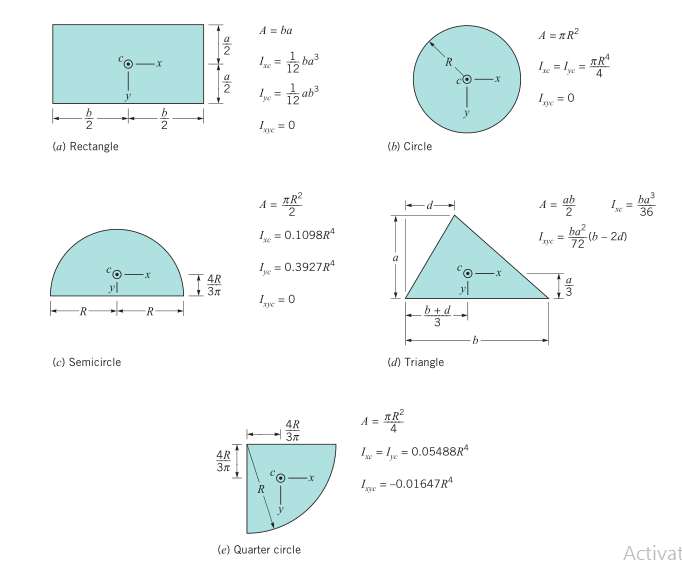
\includegraphics{Capture.png}
\caption{Moment of inertias for some systems}
\label{overflow}
\end{figure}
\end{document}